\documentclass[a4paper,12pt]{article}
\usepackage[utf8]{inputenc}
\usepackage[spanish]{babel}
\usepackage{amsmath}
\usepackage{siunitx}
\usepackage{geometry}
\usepackage{booktabs}
\usepackage{graphicx}
\usepackage{caption}
\usepackage{circuitikz}

\geometry{margin=2.5cm}
\sisetup{per-mode=symbol, separate-uncertainty=true}

\begin{document}

%--------------------------------------------------
% Carátula
%--------------------------------------------------
\begin{titlepage}
    \centering
    \vspace*{2cm}
    \textbf{\Large Instituto Tecnológico de Buenos Aires} \\
    \vspace{0.5cm}
    \textbf{\large Física III} \\
    \vspace{1cm}
    \textbf{\LARGE Trabajo Práctico N°3 (Primera Parte): Circuito RLC serie} \\
    \vspace{1.5cm}
    \begin{tabular}{ll}
        \textbf{Grupo:} & \textit{3} \\
        \textbf{Integrantes:} & \textit{Pinausig Castillo, Tomás (63167)} \\
                              & \textit{Peral Belmont, Javier (62108)} \\
                              & \textit{Ferrari, Franco (63094)} \\
                              & \textit{Lopez Denegri, Agustina (64781)} \\
        \textbf{Fecha de realización:} & \textit{Viernes 31 de Octubre} \\
        \textbf{Fecha de entrega:} & \textit{Viernes 14 de Noviembre} \\
    \end{tabular}
    \vspace{2cm}
    \begin{tabular}{|p{12cm}|}
        \hline
        \textbf{Observaciones del docente:} \\
        \vspace{5cm} \\
        \hline
    \end{tabular}
    \vspace{1cm}
    \begin{tabular}{p{6cm}}
        \textbf{Firma del docente:} \\
        \vspace{1cm} \\
        \hrule
    \end{tabular}
\end{titlepage}

%--------------------------------------------------
\section{Objetivos y Resumen}
%--------------------------------------------------
Este trabajo práctico corresponde a la \textbf{primera parte} de la consigna, dedicada exclusivamente al estudio de un \textbf{circuito RLC serie} excitado por una fuente de tensión senoidal.

Los objetivos principales fueron:
\begin{itemize}
    \item Montar un circuito RLC serie con una resistencia conocida \( R \), un capacitor \( C \) y una bobina \( L \), alimentado por un generador de funciones.
    \item Medir la tensión sobre la resistencia en función de la frecuencia de la fuente, identificando la \textbf{frecuencia de resonancia} \( f_0 \).
    \item Determinar experimentalmente la \textbf{inductancia} \( L \) a partir de la frecuencia de resonancia y de la capacitancia conocida.
    \item Estimar el \textbf{factor de calidad} \( Q \) mediante el ancho de banda en torno a la resonancia y compararlo con la expresión teórica.
    \item Discutir la influencia de la resistencia y de las pérdidas sobre la selectividad del circuito, así como las principales fuentes de error experimental.
\end{itemize}

En el experimento, se utilizó una resistencia de \( R = \SI{67}{\ohm} \) y un capacitor de \( C = \SI{194e-9}{\farad} \). A partir de la curva de tensión en la resistencia en función de la frecuencia, se identificó una frecuencia de resonancia aproximadamente igual a \( f_0 \approx \SI{4.18e3}{\hertz} \), de la cual se obtuvo una inductancia experimental \( L_{\text{exp}} \approx \SI{7.5e-3}{\henry} \). El factor de calidad resultó \( Q_{\text{exp}} \approx 0.94 \), mientras que la expresión teórica da \( Q_{\text{teo}} \approx 2.9 \), lo que indica un circuito fuertemente amortiguado, con pérdidas adicionales asociadas principalmente a la resistencia de la bobina y del cableado. Estos resultados se discuten en detalle a continuación.

%--------------------------------------------------
\section{Introducción Teórica}
%--------------------------------------------------
\subsection{Circuito RLC serie y resonancia}
Un circuito RLC serie está formado por una resistencia \( R \), una inductancia \( L \) y una capacitancia \( C \) conectadas en serie a una fuente de tensión alterna
\[
V(t) = V_0 \sin(\omega t),
\]
con frecuencia angular \( \omega = 2\pi f \). La \textbf{impedancia} total del circuito es
\[
Z(\omega) = R + j\left(\omega L - \frac{1}{\omega C}\right),
\]
de modo que el módulo de la corriente es
\[
I(\omega) = \frac{V_0}{\lvert Z(\omega)\rvert}
          = \frac{V_0}{\sqrt{R^2 + \left(\omega L - \dfrac{1}{\omega C}\right)^2}}.
\]

La reactancia inductiva \( X_L = \omega L \) crece con la frecuencia, mientras que la reactancia capacitiva \( X_C = 1/(\omega C) \) decrece con la frecuencia. Para cierta frecuencia \textbf{de resonancia} \( \omega_0 \), se cumple la condición de cancelación de reactancias:
\[
\omega_0 L = \frac{1}{\omega_0 C}
\quad \Rightarrow \quad
\omega_0 = \frac{1}{\sqrt{LC}},
\]
y por lo tanto
\[
f_0 = \frac{\omega_0}{2\pi} = \frac{1}{2\pi\sqrt{LC}}.
\]
En resonancia, la impedancia es puramente resistiva (\( Z = R \)) y la corriente alcanza su valor máximo:
\[
I_0 = \frac{V_0}{R}.
\]
La tensión sobre la resistencia, que es la magnitud medida experimentalmente, vale
\[
V_R(\omega) = I(\omega)\,R,
\]
por lo que el máximo de \( V_R \) coincide con la condición de resonancia del circuito.

\subsection{Ancho de banda y factor de calidad}
Para caracterizar qué tan ``selectivo'' es el circuito alrededor de la resonancia se define el \textbf{factor de calidad} \( Q \). En un circuito RLC serie, puede expresarse de dos maneras equivalentes:
\begin{align}
Q &= \frac{\omega_0 L}{R} = \frac{1}{R}\sqrt{\frac{L}{C}}, \\
Q &= \frac{f_0}{\Delta f},
\end{align}
donde \( \Delta f = f_2 - f_1 \) es el \textbf{ancho de banda} entre las frecuencias \( f_1 \) y \( f_2 \) definidas por la condición
\[
I(f_1) = I(f_2) = \frac{I_0}{\sqrt{2}},
\]
es decir, donde la potencia disipada en la resistencia cae a la mitad del valor máximo (frecuencias de \(-3\,\si{\decibel}\)). Un valor grande de \( Q \) implica un pico angosto de resonancia (circuito poco amortiguado y muy selectivo), mientras que un \( Q \) cercano a 1 indica un circuito fuertemente amortiguado, con un máximo más ancho.

En la práctica, las pérdidas adicionales debidas a la resistencia interna de la bobina, al cableado y a la propia fuente de señal incrementan la resistencia efectiva del circuito, disminuyendo el valor experimental de \( Q \) respecto del valor ideal calculado con la resistencia nominal.

%--------------------------------------------------
\section{Instrumentos y Elementos Empleados}
%--------------------------------------------------
Para la realización del experimento de la primera parte se utilizaron los siguientes elementos:
\begin{itemize}
    \item Resistencia \( R = \SI{67}{\ohm} \).
    \item Capacitor \( C = \SI{194e-9}{\farad} \) (\SI{194}{\nano\farad}).
    \item Inductor (bobina) utilizado para conformar el circuito RLC serie.
    \item Generador de funciones (señal senoidal de frecuencia variable y amplitud aproximadamente constante).
    \item Osciloscopio digital para medir la tensión sobre la resistencia.
    \item Multímetro para verificar valores de tensión y continuidad.
    \item Protoboard y cables de conexión.
\end{itemize}

\begin{figure}[h]
    \centering
    % Reemplazar por una foto real del montaje del circuito
    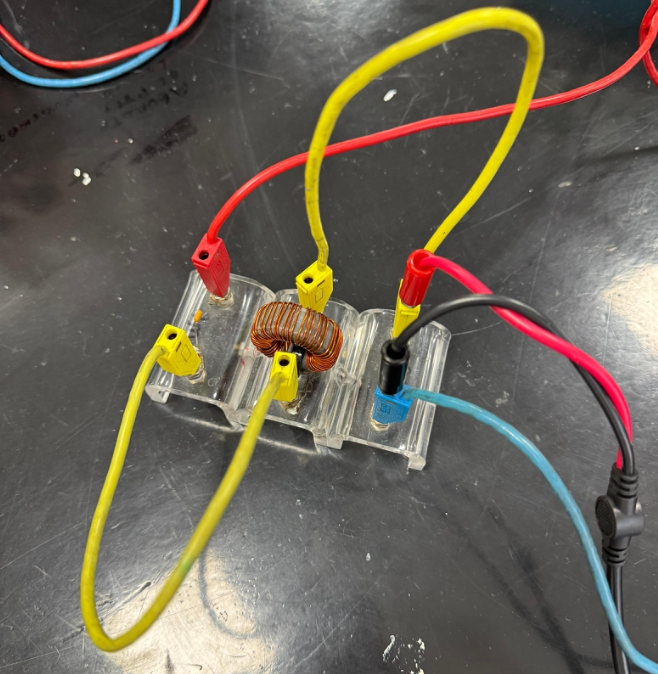
\includegraphics[width=0.4\textwidth]{CircuitoRLC.png}
    \caption{Montaje experimental del circuito RLC serie.}
\end{figure}

Adicionalmente, se utilizó un software de planilla de cálculo para procesar los datos numéricos registrados y generar los gráficos de \( V_R \) en función de la frecuencia.

%--------------------------------------------------
\section{Procedimiento Experimental}
%--------------------------------------------------
\subsection{Armado del circuito}
Se armó un circuito RLC serie conectando en serie la resistencia \( R \), la bobina \( L_1 \) y el capacitor \( C \), todos ellos alimentados por la salida del generador de funciones. La tensión a medir fue la caída de potencial sobre la resistencia, conectando las puntas del osciloscopio en paralelo con ella.

La configuración esquemática del circuito fue:
\begin{figure}[h]
    \centering
    \begin{circuitikz}
        \draw
        (0,0) to[sinusoidal voltage source, l=$V(t)$] (0,2)
        to[R=$R$] (2,2)
        to[L=$L_1$] (4,2)
        to[C=$C$] (6,2)
        to[short] (6,0)
        to[short] (0,0);
    \end{circuitikz}
    \caption{Esquema del circuito RLC serie utilizado en el experimento.}
\end{figure}

\subsection{Búsqueda de la frecuencia de resonancia}
Con el circuito armado, se fijó una amplitud de salida del generador y se barrió la frecuencia de la señal senoidal en un rango de algunos kilohertz. Para cada frecuencia se observó la amplitud de la señal de tensión sobre la resistencia en el osciloscopio.

Se identificó la frecuencia para la cual la amplitud de \( V_R \) alcanzó un máximo. Esta frecuencia se registró como \textbf{frecuencia de resonancia experimental} \( f_{0,\text{exp}} \). Los datos correspondientes se registraron en la planilla de laboratorio, quedando consignado un valor cercano a \( f_{0,\text{exp}} \approx \SI{4.0e3}{\hertz} \).

\begin{figure}[h]
    \centering
    % Reemplazar por una captura real del osciloscopio en resonancia
    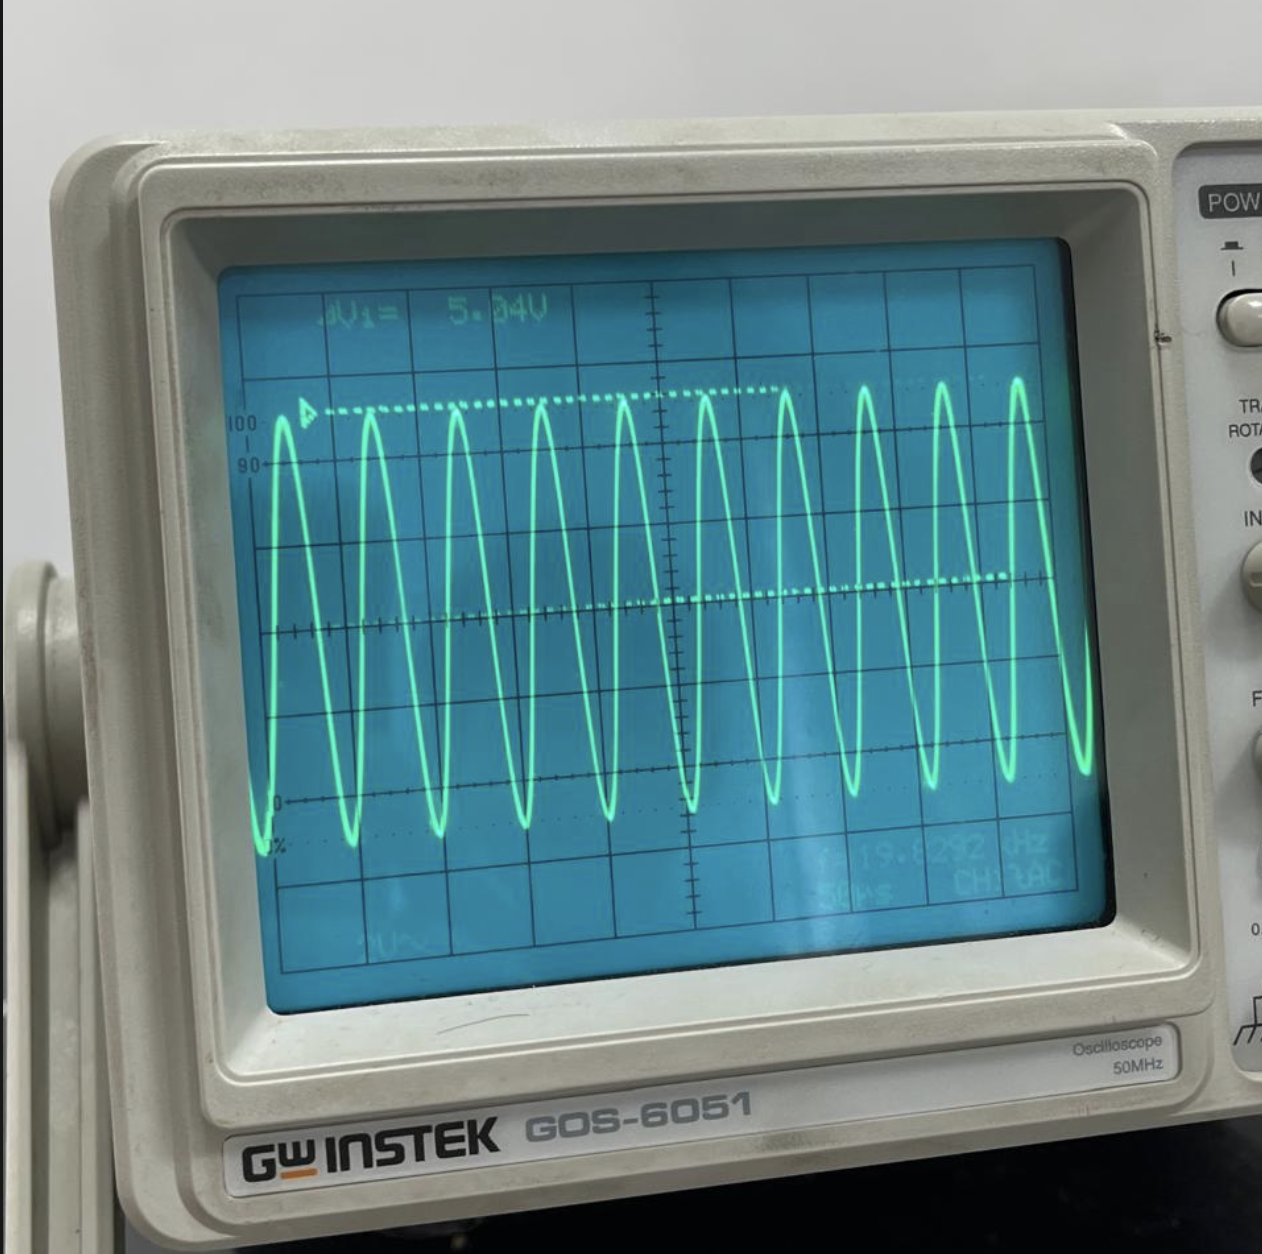
\includegraphics[width=0.4\textwidth]{Osciloscopio.png}
    \caption{Captura de pantalla del osciloscopio mostrando la tensión en la resistencia en la frecuencia de resonancia.}
\end{figure}

\subsection{Obtención de la curva \( V_R(f) \)}
Una vez localizado el entorno de resonancia, se realizó un barrido más detallado de frecuencia. Para cada valor de frecuencia \( f \) se midió la amplitud máxima de la señal de tensión sobre la resistencia, \( V_R \), y se registraron los datos en la planilla.

En particular, se tomaron medidas desde frecuencias mayores que la de resonancia hasta frecuencias menores, con pasos más finos alrededor del máximo. Con estos datos se construyó posteriormente la curva \( V_R(f) \) para analizar cuantitativamente la resonancia y estimar el factor de calidad \( Q \).

Además, se identificaron dos frecuencias \( f_1 \) y \( f_2 \) asociadas aproximadamente a la condición de media potencia, es decir, aquellas para las cuales la tensión en la resistencia se reduce a un valor cercano a \( V_{R,\text{max}}/\sqrt{2} \).

\begin{figure}[h]
    \centering
    % Reemplazar por el gráfico real obtenido a partir de la planilla de cálculo
    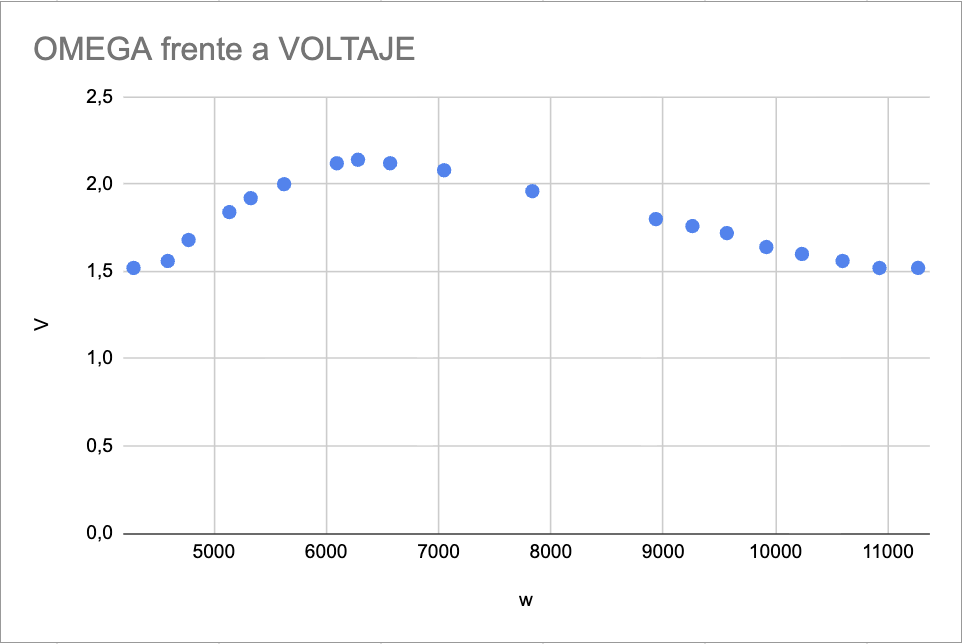
\includegraphics[width=0.8\textwidth]{Grafico.png}
    \caption{Tensión en la resistencia en función de la frecuencia, mostrando el máximo de resonancia.}
\end{figure}

%--------------------------------------------------
\section{Datos Obtenidos: Discusión y Cálculo de Errores}
%--------------------------------------------------
\subsection{Parámetros del circuito}
Durante la experiencia se trabajó con los siguientes parámetros del circuito:

\begin{table}[h]
    \centering
    \begin{tabular}{lll}
        \toprule
        Magnitud & Símbolo & Valor \\
        \midrule
        Resistencia & \( R \) & \SI{67}{\ohm} \\
        Capacitancia & \( C \) & \SI{194e-9}{\farad} \\
        Frecuencia de resonancia experimental & \( f_{0,\text{exp}} \) & \(\approx \SI{4.18e3}{\hertz}\) \\
        \bottomrule
    \end{tabular}
    \caption{Parámetros del circuito RLC serie utilizados en el experimento.}
\end{table}

\subsection{Tensión en la resistencia en función de la frecuencia}
Durante el barrido de frecuencia se registraron los valores de la tensión máxima sobre la resistencia \( V_R \) para distintos valores de frecuencia en el entorno de la resonancia. A continuación se presenta una tabla resumen con las mediciones relevantes:

\begin{table}[h]
    \centering
    \begin{tabular}{ccc}
        \toprule
        Frecuencia \( f \) [Hz] & Comentario & \( V_R \) [V] \\
        \midrule
        7174 & \( f_2 \) (alta) & 1{,}52 \\
        6955 & & 1{,}52 \\
        6746 & & 1{,}56 \\
        6516 & & 1{,}60 \\
        6314 & & 1{,}64 \\
        6090 & & 1{,}72 \\
        5895 & & 1{,}76 \\
        5688 & & 1{,}80 \\
        4988 & & 1{,}96 \\
        4488 & & 2{,}08 \\
        4182 & \( f_0 \) (resonancia) & 2{,}12 \\
        4000 & & 2{,}14 \\
        3880 & & 2{,}12 \\
        3581 & & 2{,}00 \\
        3392 & & 1{,}92 \\
        3271 & & 1{,}84 \\
        3040 & & 1{,}68 \\
        2922 & \( f_1 \) (baja, calculada) & 1{,}56 \\
        2728 & \( f_1 \) (baja) & 1{,}52 \\
        \bottomrule
    \end{tabular}
    \caption{Tensión máxima medida sobre la resistencia en función de la frecuencia, en el entorno de la resonancia.}
\end{table}

A partir de estos datos se construyó el gráfico \( V_R(f) \) mostrado en la figura correspondiente. Se observa un máximo amplio en el entorno de \( f_0 \approx \SI{4.18e3}{\hertz} \), con una caída gradual de la amplitud a ambos lados de la resonancia, característica de un circuito RLC serie con amortiguamiento significativo.

\subsection{Determinación de la inductancia a partir de la resonancia}
Utilizando la condición de resonancia para un circuito RLC serie,
\[
f_0 = \frac{1}{2\pi\sqrt{LC}},
\]
es posible despejar la inductancia:
\[
L_{\text{exp}} = \frac{1}{(2\pi f_0)^2 C}.
\]

Tomando como frecuencia de resonancia el valor obtenido de las mediciones \( f_0 = \SI{4182}{\hertz} \), y la capacitancia \( C = \SI{194e-9}{\farad} \), se obtiene:
\[
L_{\text{exp}} = \frac{1}{\bigl(2\pi \cdot 4182\bigr)^2 \cdot 194\times 10^{-9}}
               \approx \SI{7.5e-3}{\henry}
               = \SI{7.5}{\milli\henry}.
\]
Este valor de \( L_{\text{exp}} \) es coherente con un inductor de unas pocas milésimas de henry.

\subsection{Cálculo del factor de calidad}
El factor de calidad puede estimarse a partir de las frecuencias \( f_1 \) y \( f_2 \) que delimitan el ancho de banda. De la planilla se obtienen:
\[
f_1 \approx \SI{2728}{\hertz}, \qquad
f_2 \approx \SI{7174}{\hertz}.
\]

El ancho de banda experimental es entonces:
\[
\Delta f = f_2 - f_1 \approx 7174 - 2728 = \SI{4446}{\hertz},
\]
y el factor de calidad experimental resulta:
\[
Q_{\text{exp}} = \frac{f_0}{\Delta f}
               \approx \frac{4182}{4446}
               \approx 0.94.
\]

Por otro lado, utilizando la expresión teórica para un circuito RLC serie ideal:
\[
Q_{\text{teo}} = \frac{1}{R}\sqrt{\frac{L_{\text{exp}}}{C}},
\]
y sustituyendo \( R = \SI{67}{\ohm} \), \( L_{\text{exp}} \approx \SI{7.5e-3}{\henry} \) y \( C = \SI{194e-9}{\farad} \), se obtiene:
\[
Q_{\text{teo}} \approx 2.9.
\]

La discrepancia entre \( Q_{\text{exp}} \approx 0.94 \) y \( Q_{\text{teo}} \approx 2.9 \) indica que el circuito real presenta pérdidas adicionales. En particular, la resistencia efectiva del circuito es mayor que la resistencia nominal de \SI{67}{\ohm}, debido a la resistencia interna de la bobina, las pérdidas en el núcleo (si lo tuviera) y la resistencia de los cables y contactos. Esto produce un ensanchamiento del pico de resonancia y una reducción del valor de \( Q \) medido.

\subsection{Fuentes de error e incertidumbre}
Entre las principales fuentes de error que pueden afectar los resultados se encuentran:
\begin{itemize}
    \item \textbf{Resolución en la medición de la frecuencia}: el generador de funciones y/o el osciloscopio tienen una resolución finita en frecuencia, lo que introduce incertidumbre en la determinación precisa de \( f_0 \), \( f_1 \) y \( f_2 \).
    \item \textbf{Lectura de tensiones en el osciloscopio}: la estimación de la amplitud \( V_R \) se ve afectada por el grosor de las trazas, el ruido y la calibración del canal vertical.
    \item \textbf{Variaciones en la amplitud de la fuente}: idealmente la amplitud \( V_0 \) del generador debería ser constante con la frecuencia, pero en la práctica puede variar ligeramente, modificando la altura del pico de resonancia.
    \item \textbf{Resistencias parásitas}: la presencia de resistencia en la bobina y en los cables aumenta la resistencia efectiva, reduciendo \( Q \) respecto del valor ideal.
    \item \textbf{Tolerancias de los componentes}: los valores nominales de \( R \) y \( C \) tienen tolerancias típicas de algunos por ciento, lo que afecta la predicción teórica de \( f_0 \) y \( Q \).
\end{itemize}

Una estimación más detallada de las incertidumbres requeriría disponer de los errores absolutos de \( R \), \( C \), \( f \) y \( V_R \), información que no se encontraba completamente especificada durante la experiencia. No obstante, cualitativamente puede afirmarse que la diferencia entre \( Q_{\text{exp}} \) y \( Q_{\text{teo}} \) está dominada por las pérdidas resistivas adicionales del circuito real.

%--------------------------------------------------
\section{Análisis de los Resultados Obtenidos}
%--------------------------------------------------
Los resultados muestran que el circuito RLC serie estudiado presenta una frecuencia de resonancia experimental en el orden de los \SI{4e3}{\hertz}, en acuerdo razonable con la expectativa para los valores de \( R \) y \( C \) utilizados. La inductancia efectiva determinada a partir de la condición de resonancia, \( L_{\text{exp}} \approx \SI{7.5}{\milli\henry} \), es físicamente plausible y permite reconciliar los datos experimentales con la teoría.

El análisis del ancho de banda y del factor de calidad indica que el circuito se encuentra significativamente amortiguado: \( Q_{\text{exp}} \approx 0.94 \) es sensiblemente menor que el valor ideal \( Q_{\text{teo}} \approx 2.9 \). Esta diferencia se explica por la presencia de resistencias parásitas y por las pérdidas propias de un montaje real, que no se incluyen en el modelo ideal.

El gráfico de \( V_R \) en función de la frecuencia evidencia un pico relativamente ancho, típico de un circuito con amortiguamiento fuerte. Esto implica que el circuito no es altamente selectivo, lo cual puede ser una desventaja en aplicaciones de filtrado muy estrecho, pero resulta aceptable para aplicaciones donde se requiere un ancho de banda mayor.

%--------------------------------------------------
\section{Aplicaciones Prácticas}
%--------------------------------------------------
Los circuitos RLC serie se utilizan ampliamente como \textbf{filtros pasa-banda} en aplicaciones de radiofrecuencia y audio. Ajustando los valores de \( L \) y \( C \), es posible seleccionar la frecuencia de resonancia para sintonizar una banda específica de frecuencias, como ocurre en los sintonizadores de radio y en ciertos filtros de instrumentos de medida.

En electrónica de potencia y en fuentes de alimentación conmutadas, los circuitos resonantes se emplean para reducir el contenido armónico de la corriente o de la tensión, mejorando la eficiencia y disminuyendo el ruido electromagnético. En instrumentación y mediciones, los circuitos RLC permiten seleccionar o rechazar determinadas frecuencias, por ejemplo en filtros de línea o en etapas de acondicionamiento de señal.

El estudio experimental realizado en este trabajo práctico constituye una introducción a estos conceptos, mostrando cómo las magnitudes medidas en el laboratorio (tensión en la resistencia, frecuencias de resonancia y de media potencia) se vinculan con parámetros de diseño como \( L \), \( C \) y \( Q \).

%--------------------------------------------------
\section{Conclusión}
%--------------------------------------------------
En esta primera parte del Trabajo Práctico N°3 se analizó el comportamiento de un circuito RLC serie alimentado por una fuente senoidal. A partir de las mediciones de la tensión sobre la resistencia en función de la frecuencia, se determinó una frecuencia de resonancia \( f_0 \approx \SI{4.18e3}{\hertz} \) y una inductancia efectiva \( L_{\text{exp}} \approx \SI{7.5}{\milli\henry} \), en buena concordancia con la teoría cualitativa del circuito.

El cálculo del factor de calidad mostró un valor experimental \( Q_{\text{exp}} \approx 0.94 \), significativamente menor que el valor ideal estimado \( Q_{\text{teo}} \approx 2.9 \), lo que evidencia el efecto de las pérdidas resistivas adicionales presentes en el montaje real. Estas pérdidas ensanchan el pico de resonancia y reducen la selectividad del circuito.

En conjunto, el trabajo permitió relacionar las mediciones de laboratorio con los modelos teóricos estudiados en la asignatura, comprendiendo el rol de los parámetros \( R \), \( L \) y \( C \) en la respuesta en frecuencia de un circuito RLC serie y resaltando la importancia de considerar las no idealidades de los componentes en cualquier diseño experimental o tecnológico real.

\end{document}

